\documentclass[aps,pra,10pt,onecolumn,superscriptaddress,amsmath,amssymb]{revtex4-2}
\usepackage{graphicx}
\usepackage{bm}
\usepackage[colorlinks,allcolors=blue]{hyperref}
\newcommand{\Lc}{\mathcal L}
\newcommand{\Tr}{\operatorname{Tr}}
\renewcommand{\theequation}{S\arabic{equation}}
\renewcommand{\thefigure}{S\arabic{figure}}
\renewcommand{\thetable}{S\arabic{table}}
\begin{document}
\title{Supplemental Material for ``Finite-size decay-mode hybridization near a mean-field fold in an open Rydberg ensemble''}
\date{\today}
\maketitle

\section{Generator, symmetry sector, and precision}
We use $\gamma=1$, $\Omega=2$, and $V=10$ unless stated otherwise. A permutation-invariant operator on $N$ spin-$1/2$ particles has the form
\begin{equation}
 \rho=\bigoplus_j\frac{\widetilde\rho_j}{d_j}\otimes I_{d_j},\qquad
 d_j=\binom{N}{N/2-j}-\binom{N}{N/2-j-1},
 \label{eq:block}
\end{equation}
where a binomial coefficient with lower argument $-1$ is zero. The stored PIQS blocks $\widetilde\rho_j$ sum over representation multiplicities. The trace is $\sum_j\Tr\widetilde\rho_j$, and the number of stored entries is $\sum_j(2j+1)^2=\binom{N+3}{3}$. Local decay mixes different $j$ blocks. All spectral and dynamical claims in the paper refer to this complete permutation-invariant operator space, not only $j=N/2$ and not to other permutation-symmetry sectors.

The Hamiltonian commutator is formed by column-major vectorization, $-i(I\otimes H-H^T\otimes I)$, followed by restriction to the Dicke blocks. The independent-emission coefficients follow the PIQS formulas~\cite{Shammah2018}, evaluated in double precision in \texttt{biorthogonal\_generator.py}. For a target entry $(j,m,m')$, the diagonal decay coefficient is $-[N+(m+m')]/2$. Its off-diagonal sources have labels $(a,m_s,m_s')=(j+\delta j,m+1,m'+1)$, with $\delta j=0,+1,-1$. Their coefficients are, respectively,
\begin{align}
 \frac12\sqrt{(a+m_s)(a-m_s+1)(a+m_s')(a-m_s'+1)}
       \frac{N/2+1}{a(a+1)},\nonumber\\
 \frac12\sqrt{(a+m_s)(a+m_s-1)(a+m_s')(a+m_s'-1)}
       \frac{N/2+a+1}{a(2a+1)},\nonumber\\
 \frac12\sqrt{(a-m_s+1)(a-m_s+2)(a-m_s'+1)(a-m_s'+2)}
       \frac{N/2-a}{(a+1)(2a+1)}.
 \label{eq:emission}
\end{align}
Only allowed source labels contribute; the first two expressions vanish when their denominators refer to an unavailable zero-spin transition. These coefficients are expressed in the multiplicity-summed storage convention.

An independent small-$N$ check starts from the $2^N$-dimensional spin Hilbert space with individual jump operators, and projects the full Liouvillian onto orthonormal symmetrized Pauli strings. The maximal matched spectral differences are shown in Table~\ref{tab:small}. This verifies the generator separately from eigensolver residuals, which cannot detect a common error in the matrix itself.

\begin{table}[h]
\caption{Independent full-spin versus Dicke-block generator check. The invariance residual tests the full-spin action on the symmetrized Pauli basis.}
\label{tab:small}
\begin{ruledtabular}
\begin{tabular}{rrrr}
$N$&Dimension&Maximum spectral difference&Invariance residual\\
1&4&$1.99\times10^{-15}$&$1.02\times10^{-15}$\\
2&10&$1.01\times10^{-14}$&$1.57\times10^{-15}$\\
3&20&$3.77\times10^{-14}$&$6.01\times10^{-15}$\\
4&35&$4.46\times10^{-14}$&$2.33\times10^{-14}$
\end{tabular}
\end{ruledtabular}
\end{table}

This precision choice matters for a small gap. In the earlier PIQS-backed implementation used for exploratory calculations, internal emission coefficients led to a trace defect of approximately $4.7\times10^{-7}$ at $N=56$. The double-precision implementation reduces this to approximately $7.1\times10^{-15}$ and changes that half-gap from $0.0003260261$ to $0.0003309798$. The finite-window gap exponent changes only from $0.140624$ to $0.140501$, but all figures retained in the present paper use the double-precision results. Earlier multi-drive quasipotential tests are not used as quantitative evidence in this manuscript.

\section{Mean-field Jacobian and interpretation of the fold}
For the Bloch coordinates $q=(n,u,v)$ of the main text, the Jacobian is
\begin{equation}
 J=\begin{pmatrix}
 -1&0&-\Omega\\
 Vv&-1/2&-(\Delta-Vn)\\
 \Omega-Vu&\Delta-Vn&-1/2
 \end{pmatrix}.
\end{equation}
At stationarity, $v=-n/\Omega$ and $u=2n(\Delta-Vn)/\Omega$. Substituting these relations into $\det(\lambda I-J)$, and reducing its difference from $\lambda[(\lambda+1)^2+\Omega^2/2]$ by the polynomial constraints $F=F_n=0$, gives zero identically. This is implemented symbolically in \texttt{pra\_meanfield.py} and also checked numerically at both folds. For the parameters of the paper, the right fold is $(\Delta,n)=(4.5749637137,0.4305200135)$; both folds have Jacobian eigenvalues $0,-1\pm i\sqrt2$ to numerical precision.

The simple zero eigenvalue describes the linearization at the coalescing fixed points. The stationary cubic has a higher-order root at the cusp, but this does not change the algebraic multiplicity of the zero root in the displayed Jacobian polynomial. None of these identities identifies a finite-$N$ spectral pair with a universal escape problem.

\section{Construction and validation of physical preparations}
Let a strictly positive single-atom density matrix have Bloch vector $\bm b$, with $r=|\bm b|<1$. In the spin convention used by PIQS, the coordinates of the main text give
\begin{equation}
 \bm b=(2u,-2v,2n-1),\qquad
 \rho_1=\sqrt{\det\rho_1}\,\exp[\operatorname{arctanh}(r)\,\widehat{\bm b}\cdot\bm\sigma].
\end{equation}
The multiplicity-summed blocks of its product state are therefore
\begin{equation}
 \widetilde\rho_j=d_j(\det\rho_1)^{N/2}
       \exp[2\operatorname{arctanh}(r)\,\widehat{\bm b}\cdot\bm J_j].
 \label{eq:product}
\end{equation}
We diagonalize the Hermitian exponent within each block and evaluate the scalar weights in logarithmic form. This avoids constructing a $2^N\times2^N$ density matrix. The trace is checked before normalization.

For $N=1,2,4$, the resulting excitation-number distribution agrees with $\binom Nk n^k(1-n)^{N-k}$ to less than $1.7\times10^{-16}$, and the reconstructed single-atom coherences agree to less than $1.2\times10^{-16}$. Positivity follows directly from Eq.~\eqref{eq:product}; the single-atom states used in the calculations are strictly inside the Bloch ball. A separate $N=1$--$4$ test starts from explicit tensor products and individual spin jumps, and integrates the full-spin equation with an adaptive DOP853 solver. At $t=0,0.25,0.75,1.5$, its excitation density and purity agree with Dicke-block exponential multiplication to less than $2\times10^{-12}$. This checks the preparation and physical trace convention in time evolution, independently of the spectral comparison in Table~\ref{tab:small}.

The high-branch difference is
\begin{equation}
 \delta\rho_{\rm hi}=\rho_1(q_{\rm hi}+\eta e_{\rm hi})^{\otimes N}
                    -\rho_1(q_{\rm hi}-\eta e_{\rm hi})^{\otimes N},
\end{equation}
where $q_{\rm hi}$ is the surviving high mean-field fixed point, $e_{\rm hi}$ is its Euclidean-normalized real relaxation eigenvector with positive population component, and $\eta=0.005$. The second difference is
\begin{equation}
 \delta\rho_f=\rho_1(q_f)^{\otimes N}-\rho_{\rm ss}(\Delta),
 \qquad q_f=(0.15692704,0.31861940,-0.07846352).
\end{equation}
The fold state is fixed while $\Delta$ is varied. It is not asserted to be a stationary or metastable state of the finite generator at those detunings.

For each detuning the real spectral pair is computed together with its transpose-left dual. If $H=W_d^TLR_d$ is the diabatic representation, diagonalizing $H=T\Lambda T^{-1}$ gives eigenmode bases $R=R_dT$ and $W=W_d(T^{-1})^T$. The observable residues are calculated from these exact eigenmode bases, not from the diagonal entries of the diabatic matrix. Scanning 15 detunings over $\Delta_*(32)\pm0.06$ resolves the transfer of response; the endpoints and crossing are separately evaluated for $N=40$. The largest right invariant-subspace residual in the $N=32$ scan is $1.46\times10^{-12}$.

At $N=32$, changing the ARPACK seed and shift from $-0.76$ to $-0.80$ changes the two real eigenvalues at the three diagnostic detunings by less than $9.0\times10^{-15}$. Halving $\eta$ changes the residue vector divided by $2\eta$ by $4.96\times10^{-6}$, $7.29\times10^{-6}$, and $5.75\times10^{-6}$ in relative Euclidean norm, respectively. These checks support the perturbative interpretation of the first preparation. They do not turn the second, finite displacement into a linearized mean-field trajectory.

\section{Biorthogonal projection and normalization conventions}
The left eigenvectors are computed from $L^T$. In column-major vectorization the bilinear pairing $W^TR$ is the algebraic dual; physical observables are represented with the corresponding transpose. For a real decay mode of a Hermiticity-preserving generator, we phase-align and Hermitize the right and dual left eigenoperators, then enforce $W^TR=I$ in the selected two-dimensional subspace. Eigensolver, Hermiticity, trace, and subspace residuals are retained separately.

In this basis the derivative matrix $W^TL_1R$ has two distinct real eigenvalues. Diagonalizing it defines the local diabatic modes. At the projection point, the derivative of the two-eigenvalue discriminant is unaffected by basis-derivative commutators. This gives the stationarity identity used in the main text. Numerically, the minimum is refined using
\begin{equation}
 \delta\Delta=-\frac{e_a-e_b}{s_a-s_b}
\end{equation}
until $|\delta\Delta|<10^{-11}$, with independently checked eigenmode and subspace residuals.

Let $P=R_dW_d^T$ be the generally oblique spectral projector at $\Delta_*$ and $Q=I-P$. Since $P$ commutes with $L_*=L(\Delta_*)$, the exact spectral effective matrix away from that point is
\begin{align}
 H_{\rm eff}(z,\delta)={}&H_P(\delta)\nonumber\\
 &+\delta^2 W_d^TL_1Q
 [z-Q(L_*+\delta L_1)Q]^{-1}_{Q}QL_1R_d.
 \label{eq:Qcorrection}
\end{align}
The inverse acts on the range of $Q$. Thus the frozen linear matrix reproduces the value and first derivative at the reference point but not the complete neighboring spectrum. At $N=40$, over $|\delta|\le2g/|s_a-s_b|$, its largest tested half-gap relative error is $1.39\times10^{-3}$. A small absolute correction is not automatically negligible relative to a much smaller off-diagonal element.

In the stored convention of Eq.~\eqref{eq:block}, the physical trace norm of a Hermitian right operator is
\begin{equation}
 \|R\|_1=\sum_j\Tr|\widetilde R_j|.
\end{equation}
The corresponding norm of a dual observable is the maximum operator norm over its blocks. No extra representation-multiplicity factor is inserted on the left. Table~\ref{tab:gauge} lists descriptive logarithmic slopes for the same data window under different normalizations. The balanced normalization uses $c_b/c_a=\sqrt{|V_{ba}/V_{ab}|}$ and forces equal magnitudes.

\begin{table}[h]
\caption{Finite-window coupling exponents for $N=24,28,\ldots,56$. The individual values are normalization-dependent.}
\label{tab:gauge}
\begin{ruledtabular}
\begin{tabular}{lrrr}
Right-mode normalization&$\alpha_{ab}$&$\alpha_{ba}$&$(\alpha_{ab}+\alpha_{ba})/2$\\
Population peak&0.00963768&0.27136532&0.14050150\\
Physical trace norm&0.00356277&0.27744023&0.14050150\\
Balanced&0.14050150&0.14050150&0.14050150
\end{tabular}
\end{ruledtabular}
\end{table}

\section{Boundary flux and the limits of tail arguments}
For a diagonal mask $\chi$ in the stored operator coordinates, define
\begin{equation}
 J_{ab}=W_a^T[\chi,L]R_b,\qquad
 D_a=W_a^T\chi R_a,\qquad O_{ab}=W_a^T\chi R_b.
\end{equation}
The invariance equations $LR=RH$ and $W^TL=HW^T$ give
\begin{equation}
 J_{ab}=(e_b-e_a)O_{ab}+V_{ab}(D_a-D_b).
\end{equation}
At the gap minimum, $e_a=e_b$, this is a flux representation of the cross coupling. The masks used in the diagnostic are
\begin{equation}
 \chi_{(j,m,m')}=\mathbf1\!\left[\frac{k_m+k_{m'}}{2N}\le n_c\right],
 \qquad k_m=m+N/2.
\end{equation}
They are coordinate masks, not quantum channels or probabilities of measurement outcomes.

Eight cuts and nine sizes reconstruct the cross couplings with relative error below $1.6\times10^{-8}$. Nevertheless, splitting the weak flux into an absolute envelope and a cancellation factor is not invariant. For $n_c=0.157$, their fitted exponents over $N=24$--$56$ are approximately $0.13123$ and $0.13942$; at $n_c=0.30$ they become $0.01137$ and $0.25778$. The denominator correction restores the same total coupling exponent. This prevents interpreting the two contributions at one selected cut as two independently determined activation actions.

The weak-coupling contraction can also be written $W_b^T(L-e_a)R_a$. In the exact projected subspace, $(L-e_a)R_a=V_{ba}R_b$, so the small quantity is transferred from a large cancelling sum into an exponentially small residual. An asymptotic calculation must determine that residual independently; using exact spectral modes to reconstruct it is not a WKB prediction.

\section{Complex-detuning exceptional points}
We use a full-generator complex continuation $L(\zeta)=L_0+\zeta L_1$, independently of the real spectral-parameter recursion. A two-sided block inverse iteration, with QR orthonormalization, gives right and transpose-left invariant subspaces. After dual normalization, define
\begin{equation}
 H=W^TLR,\quad B=W^TL_1R,\quad
 D=\left(\frac{H_{00}-H_{11}}{2}\right)^2+H_{01}H_{10}.
\end{equation}
Because $D$ is a similarity invariant, its derivative is
\begin{equation}
 D'=\frac{(H_{00}-H_{11})(B_{00}-B_{11})}{2}
       +B_{01}H_{10}+H_{01}B_{10}.
\end{equation}
Newton iterations update both the detuning and invariant subspaces; they do not solve only a frozen two-by-two model. The QR basis remains regular at an EP, where individual eigenvectors become ill-conditioned.

\begin{table}[h]
\caption{Double-precision complex-detuning EPs. $M=H-\frac12\Tr(H)I$. Rates are in units of $\gamma$. The norm of $M$ is evaluated with an orthonormal right-subspace basis.}
\label{tab:ep}
\begin{ruledtabular}
\begin{tabular}{rccrr}
$N$&$\zeta_{\rm EP}$&$\lambda_{\rm EP}$&$\|M\|_F$&$\|M^2\|_F/\|M\|_F^2$\\
24&$3.136806063+0.026370766i$&$-0.751013173+0.031608734i$&0.25945&$2.80\times10^{-15}$\\
32&$3.205686613+0.007464558i$&$-0.755104588+0.010634053i$&0.26380&$2.10\times10^{-15}$\\
40&$3.250218904+0.002129005i$&$-0.757677321+0.003436485i$&0.26840&$3.24\times10^{-15}$
\end{tabular}
\end{ruledtabular}
\end{table}

The largest left or right subspace residual at the final EP points is $1.61\times10^{-12}$. Independent full-matrix ARPACK candidates have target-mode residuals below $1.68\times10^{-13}$. Direct eigenvalues at the EP still split by roughly $4$--$7\times10^{-8}$ in floating-point arithmetic; we do not report this as an exact zero. The nonzero nilpotent part, simple zero of $D$, and the branch exchange provide complementary local evidence. Eight nearby candidate modes are retained; the nearest sampled external-mode distance is $0.457$--$0.460$. This is not a global exclusion of other EPs or other spectral sectors.

For $N=32$, we take $\zeta(\theta)=\zeta_{\rm EP}+r e^{i\theta}$ with $r=0.00223936747$, less than the distance to the conjugate EP. At 24 points per circuit, the one-circuit exchange and two-circuit return errors are $9.75\times10^{-14}$ and $8.41\times10^{-14}$. The discriminant winds once and twice, respectively. Repeating with a different random seed, inverse-iteration shift, initial detuning, and 48 points per circuit changes the EP by $4.83\times10^{-15}$ and common-node eigenvalues by at most $2.24\times10^{-13}$. A complex-direction central difference of $D$ agrees with $D'$ to relative error $4.10\times10^{-8}$.

\begin{figure}[h]
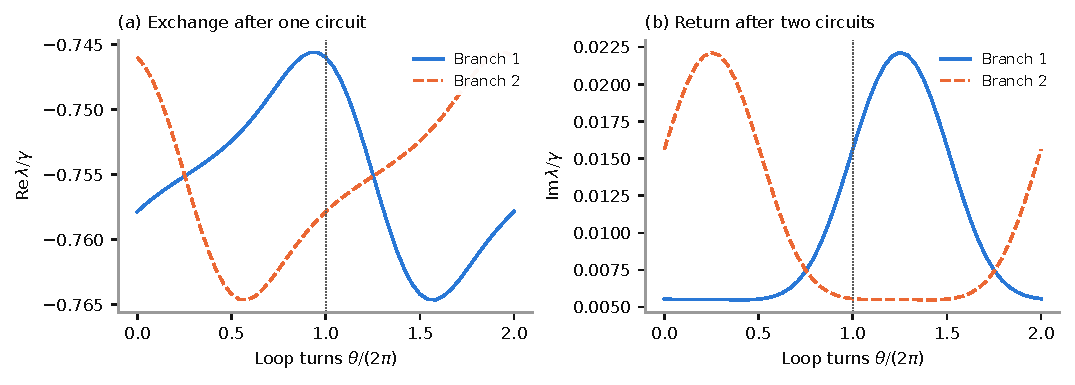
\includegraphics[width=.96\textwidth]{../figs/pra_ep_loop.pdf}
\caption{Full-generator eigenvalue continuation around the $N=32$ complex-detuning EP. Branch labels are followed continuously, rather than resorted at each point. The two branches exchange after one circuit and return after two. This complex-parameter loop is a spectral diagnostic, not a physical CPTP evolution.}
\end{figure}

\section{Coherence recursion, derivatives, and real-root validation}
For real $z$, each denominator $X_q=zI-A_q-\Sigma_q(z)$ is inverted by a linear solve. Set $G_q=X_q^{-1}$ and $E_q=I-\Sigma_q'$. Differentiation of the positive-order recursion gives
\begin{align}
 \Sigma_{q-1}'&=-U_{q-1}G_qE_qG_qD_{q-1},\\
 \Sigma_{q-1}''&=U_{q-1}\left[2G_qE_qG_qE_qG_q+G_q\Sigma_q''G_q\right]D_{q-1}.
\end{align}
With $K=A_0+2\operatorname{Re}\Sigma_0$, a simple real eigenbranch obeys
\begin{align}
 \mu'&=l^TK'r,\qquad l^Tr=1,\\
 (K-\mu I)r'&=-(K'-\mu'I)r,\qquad l^Tr'=0,\\
 \mu''&=l^TK''r+2l^TK'r'.
\end{align}
The middle equation is solved as a bordered linear system. All derivatives are with respect to the spectral variable $z$, not detuning. At the four minima $|f'|<2.3\times10^{-12}$; eigenmode and differentiated-equation residuals are below $5.1\times10^{-13}$. For $N=24$, central differences with step $10^{-4}$ agree with the first and second operator derivatives to relative errors $3.65\times10^{-8}$ and $1.53\times10^{-7}$.

The root search selects the nearest effective real eigenvalue only within the local window. Such a selection is not a global branch-tracking algorithm and can jump between branches. A final residual check is therefore mandatory. In particular, $K=\operatorname{diag}(-0.80,-0.72)$ has no self-consistent root in $[-0.78,-0.74]$, although nearest-branch selection changes sign there and can make Brent's method report convergence. The implementation rejects this false root because the final residual is about $0.04$. It also rejects a nearest effective eigenvalue with any nonzero imaginary part returned by the real-matrix eigensolver; a small complex pair is not rounded into a real root. Complex spectral inputs or detunings are rejected by the $2\operatorname{Re}\Sigma$ implementation.

For all eight retained roots, back-substitution reconstructs the complete right eigenoperator. The largest $\|LR-zR\|_2/\|R\|_2$ is $1.13\times10^{-13}$ and the largest normalized trace is $8.2\times10^{-14}$. The $q=0$ component carries between $0.360$ and $0.419$ of the full Euclidean norm. The smallest one-norm reciprocal condition estimates of the intermediate denominators at the roots range from $4.33\times10^{-4}$ to $1.73\times10^{-3}$. These checks test the computed points, not absence of poles over an entire real or complex domain. Small residuals alone are not rigorous forward-error bounds for a nonnormal matrix; the agreement with independent full-generator spectra is also retained.

\subsection{Truncating coherence orders}
Keeping only $|q|\le q_{\max}$ defines a truncated matrix, not a CPTP approximation. At low cutoffs the nearest real pair can change identity; all candidate eigenvalues are saved. Representative relative half-gap errors are given in Table~\ref{tab:cutoff}. Nonmonotonicity and different errors in the individual eigenvalues prevent treating one favorable gap value as convergence of the full spectrum.

\begin{table}[h]
\caption{Relative half-gap error from coherence truncation. Full-generator values use all $|q|\le N$.}
\label{tab:cutoff}
\begin{ruledtabular}
\begin{tabular}{rrr}
$q_{\max}$&$N=40$&$N=56$\\
8&$+5.1873$&$+165.17$\\
10&$+0.35523$&$+24.376$\\
12&$+0.025262$&$+3.7778$\\
14&$-1.704\times10^{-4}$&$+0.65009$\\
16&$-8.49\times10^{-5}$&$-2.28\times10^{-5}$\\
20&$-1.45\times10^{-5}$&$+2.35\times10^{-7}$\\
24&$-5.66\times10^{-7}$&$-1.83\times10^{-6}$
\end{tabular}
\end{ruledtabular}
\end{table}

\section{Time-domain comparison and error definitions}
The full evolution is evaluated by sparse exponential multiplication for 121 times $t=0,0.1,\ldots,12$, acting directly on the two initial differences. This avoids a time-discretized master-equation integrator. Trace conservation of the evolved differences is checked; the largest error in the three diagnostic detunings is below $9\times10^{-16}$.

The four-mode approximation includes the two real modes, the oscillatory eigenmode found near $-0.72+2.85i$, and its Hermitian-conjugate partner. Both right and transpose-left eigenmode residuals are checked. The residues are projected from the chosen preparations and observable, without fitting any time-domain parameters. For a lower time cutoff $t_0$, the reported relative error is
\begin{equation}
 E(t_0)=\frac{\left[\sum_{t\in[t_0,12]}|\delta n_{\rm approx}(t)-\delta n_{\rm full}(t)|^2\right]^{1/2}}
 {\left[\sum_{t\in[t_0,12]}|\delta n_{\rm full}(t)|^2\right]^{1/2}}.
\end{equation}
The exponential envelope removed in the figure is not removed when calculating errors. Table~\ref{tab:time} lists the $t_0=6$ comparisons. Earlier times generally contain larger contributions from omitted modes; for example, at the crossing the high-branch four-mode error is $1.49\%$ over $4\le t\le12$.

\begin{table}[h]
\caption{Relative $L^2$ errors over $6\le t\le12$ for $N=32$. All values are percentages.}
\label{tab:time}
\begin{ruledtabular}
\begin{tabular}{rrrrr}
$\Delta-\Delta_*$&High, two real&High, four modes&Fold state, two real&Fold state, four modes\\
$-0.06$&25.14&0.481&46.34&5.14\\
$0$&25.10&0.506&69.47&5.00\\
$+0.06$&25.78&0.529&4.99&0.256
\end{tabular}
\end{ruledtabular}
\end{table}

These are finite-time, preparation-dependent tests. The oscillatory pair has the less negative real part at the crossing, so it cannot be omitted solely because the target real pair has a small separation. Conversely, including four modes is not claimed to close the dynamics exactly or uniformly over all initial states.

\section{Reproduction and evidence scope}
The source bundle provides commands, scripts, JSON records, arrays, and a SHA256 manifest. The environment used Python 3.13.2, NumPy 2.2.6, SciPy 1.16.3, and QuTiP 5.3.1, with one linear-algebra thread. All calculations use \texttt{biorthogonal\_generator.py}. The stored $N=24$ coherence sample predates local geometric bracketing, and all four original root files predate the final branch-discontinuity guards. All eight roots were subsequently back-substituted with the final verifier; raw samples and source hashes preserve this provenance. Earlier quasipotential tests and unconverged instanton trajectories are not used as quantitative evidence here.

\begin{thebibliography}{9}
\bibitem{Shammah2018} N. Shammah, S. Ahmed, N. Lambert, S. De Liberato, and F. Nori, Open quantum systems with local and collective incoherent processes: Efficient numerical simulations using permutational invariance, Phys. Rev. A \textbf{98}, 063815 (2018).
\end{thebibliography}
\end{document}
